%% The Three-Rung Tower: mechanized completeness for intuitionistic,
%% Gödel--Dummett, and classical higher-order logic, with certified
%% evidence readouts.
%%
%% Build:
%%   pdflatex hol-completeness-tower.tex

\documentclass[11pt]{article}
\usepackage[T1]{fontenc}
\usepackage[utf8]{inputenc}
\usepackage{lmodern}
\usepackage{geometry}
\geometry{margin=1in}
\usepackage{hyperref}
\usepackage{booktabs}
\usepackage{array}
\usepackage{amsmath}
\usepackage{amssymb}
\usepackage{amsthm}
\usepackage{tikz}
\usetikzlibrary{arrows.meta,positioning}
\usepackage{xcolor}
\usepackage{listings}
\setlength{\emergencystretch}{3em}

\lstdefinelanguage{lean}{
  keywords={theorem, def, inductive, noncomputable, instance, structure,
    abbrev, where, fun, Prop, Type},
  sensitive=true,
  comment=[l]{--},
  morecomment=[s]{/-}{-/},
}
\lstset{
  language=lean,
  basicstyle=\footnotesize\ttfamily,
  keywordstyle=\bfseries,
  commentstyle=\itshape\color{black!60},
  columns=fullflexible,
  keepspaces=true,
  frame=leftline,
  framerule=0.6pt,
  rulecolor=\color{black!40},
  xleftmargin=1.2em,
  aboveskip=8pt, belowskip=8pt,
  literate=
    {Γ}{{$\Gamma$}}1 {Δ}{{$\Delta$}}1 {Ω}{{$\Omega$}}1
    {φ}{{$\varphi$}}1 {ψ}{{$\psi$}}1 {θ}{{$\theta$}}1 {σ}{{$\sigma$}}1
    {ρ}{{$\rho$}}1 {χ}{{$\chi$}}1 {ω}{{$\omega$}}1
    {∀}{{$\forall$}}1 {∃}{{$\exists$}}1 {∈}{{$\in$}}1 {∪}{{$\cup$}}1
    {∅}{{$\emptyset$}}1 {∧}{{$\wedge$}}1 {¬}{{$\neg$}}1
    {→}{{$\to$}}1 {↔}{{$\leftrightarrow$}}1 {⊔}{{$\sqcup$}}1
    {⊤}{{$\top$}}1 {⊥}{{$\bot$}}1 {⇨}{{$\Rightarrow$}}1
    {≠}{{$\neq$}}1 {≤}{{$\leq$}}1 {≥}{{$\geq$}}1
    {ℝ}{{$\mathbb{R}$}}1 {∞}{{$\infty$}}1 {·}{{$\cdot$}}1
}

\newcommand{\code}[1]{\texttt{#1}}
\newcommand{\BE}{\code{BinaryEvidence}}
\newcommand{\Prov}{\mathsf{Prov}}
\newcommand{\ProvLC}{\mathsf{Prov}^{\mathrm{LC}}}
\newcommand{\himp}{\Rightarrow}

\theoremstyle{plain}
\newtheorem{theorem}{Theorem}[section]
\newtheorem{lemma}[theorem]{Lemma}
\newtheorem{corollary}[theorem]{Corollary}
\theoremstyle{definition}
\newtheorem{definition}[theorem]{Definition}
\newtheorem{remark}[theorem]{Remark}

\title{The Three-Rung Tower:\\
\large Mechanized Completeness for Intuitionistic, G\"odel--Dummett, and
Classical Higher-Order Logic,\\ with Certified Evidence Readouts}
\author{Zar Goertzel\\Oru\v{z}i}
\date{\today}

\begin{document}
\maketitle

\begin{abstract}
We present a mechanized (Lean~4) development of completeness theorems for a
single natural-deduction calculus for extensional Church-style higher-order
logic at three strengths: the base calculus (intuitionistic), its extension by
the prelinearity schema (G\"odel--Dummett logic LC), and its extension by
excluded middle (classical).  All three completeness proofs share one
Lindenbaum-style spine over one class of Heyting-valued substitutional models,
and the containments between the three logics are themselves theorems,
witnessed by small concrete countermodels.  On top of the semantic core we
build a certified \emph{evidence readout} stack: proof-relevant derivation
trees with provenance and cost semantics, monotone readouts from the
derivability order into evidence carriers, and a separating-family theorem
showing that evidence comparisons provably track derivability.  A structural
highlight is a \emph{doctrine theorem}: the natural PLN evidence algebra is a
complete Heyting algebra, but using it as the truth algebra of the logic
forces the G\"odel--Dummett axiom --- so graded evidence enters intuitionistic
reasoning as a certified readout, not as primitive truth values.  Every
theorem is stated with its live mechanization name and audited axiom
footprint; the base soundness results and both canaries are choice-free.
\end{abstract}

\section{Introduction}

Reasoning systems that grade their conclusions --- probabilistic logic
networks, evidential and fuzzy reasoners, uncertain knowledge bases --- need
an answer to a foundational question: \emph{what logic do the grades live
over, and what guarantees that graded reports track the underlying
entailment?}  This paper answers the question for a mechanized higher-order
logic by building the complete semantic ladder and then the certified bridges
from proofs to grades.

The development has two halves.

\paragraph{The tower.}  One calculus --- an intrinsically typed
natural-deduction system for extensional Church-style higher-order logic,
with no excluded middle built in --- is proven sound and complete at three
strengths with respect to one class of Heyting-valued models
(Figure~\ref{fig:tower}).

\begin{figure}[t]
\centering
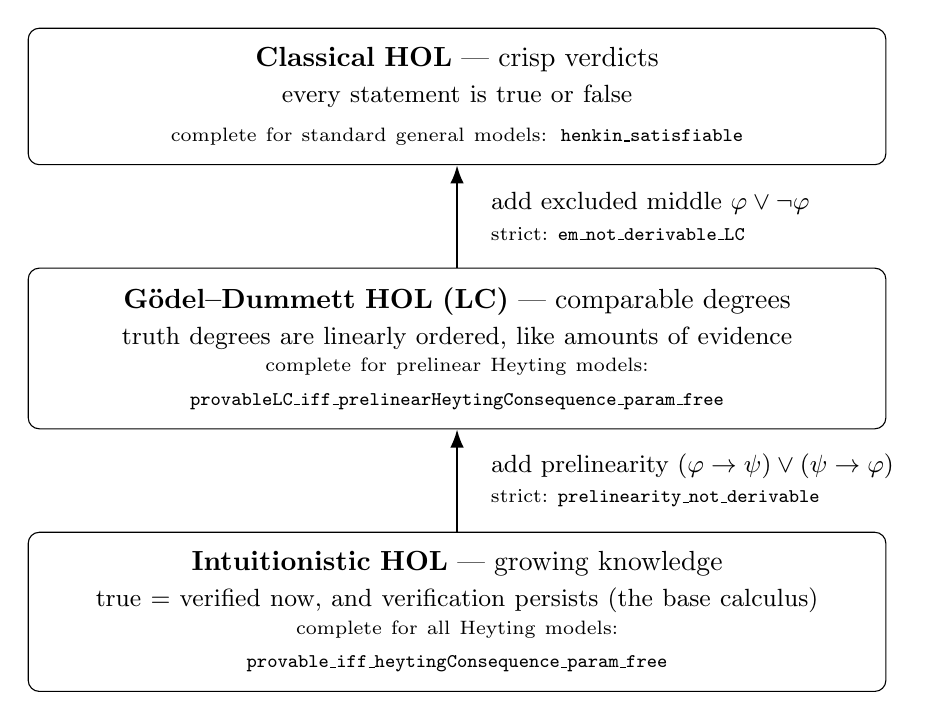
\begin{tikzpicture}[
  rung/.style={draw, rounded corners, align=center, text width=10.4cm,
    inner sep=7pt},
  climb/.style={align=left, anchor=west, xshift=3mm, font=\small}]
\node (c) [rung]
  {\textbf{Classical HOL} --- crisp verdicts\\[1pt]
   {\small every statement is true or false}\\[2pt]
   {\scriptsize complete for standard general models:
    \code{henkin\_satisfiable}}};
\node (lc) [rung, below=13mm of c]
  {\textbf{G\"odel--Dummett HOL (LC)} --- comparable degrees\\[1pt]
   {\small truth degrees are linearly ordered, like amounts of evidence}\\[2pt]
   {\scriptsize complete for prelinear Heyting models:\\
    \code{provableLC\_iff\_prelinearHeytingConsequence\_param\_free}}};
\node (i) [rung, below=13mm of lc]
  {\textbf{Intuitionistic HOL} --- growing knowledge\\[1pt]
   {\small true $=$ verified now, and verification persists (the base
    calculus)}\\[2pt]
   {\scriptsize complete for all Heyting models:\\
    \code{provable\_iff\_heytingConsequence\_param\_free}}};
\draw[-{Latex}, thick] (i) -- node[climb]
  {add prelinearity $(\varphi\to\psi)\vee(\psi\to\varphi)$\\
   {\scriptsize strict: \code{prelinearity\_not\_derivable}}} (lc);
\draw[-{Latex}, thick] (lc) -- node[climb]
  {add excluded middle $\varphi\vee\neg\varphi$\\
   {\scriptsize strict: \code{em\_not\_derivable\_LC}}} (c);
\end{tikzpicture}
\caption{The three-rung tower: one calculus, one class of Heyting-valued
models, three completeness theorems.  Climbing a rung means adopting the
axiom schema on the arrow; each climb is strict, witnessed by a concrete
countermodel that lives on the lower rung and refutes the added schema.}
\label{fig:tower}
\end{figure}

Read the tower bottom-up.  On the bottom rung, truth means
\emph{verification}: a statement holds when it has been checked, and stays
checked as knowledge grows --- so $p\vee\neg p$ is not a law, because we may
have verified neither disjunct (\code{em\_not\_derivable}, a two-world
countermodel).  On the middle rung, truth degrees behave like amounts of
evidence: any two degrees are comparable, which is precisely the prelinearity
axiom.  On the top rung every statement receives a crisp verdict.  Both
containments are \emph{strict as theorems}: a forked three-world frame
refutes prelinearity intuitionistically
(\code{prelinearity\_not\_derivable}), and a three-element G\"odel chain
refutes excluded middle inside LC (\code{em\_not\_derivable\_LC}).

\paragraph{The readouts.}  The second half connects proofs to grades.
Derivations are reified as proof-relevant trees with an axiom-free erasure to
the propositional calculus; the same tree admits multiple semiring-style
evaluations (a Boolean evaluation recovering derivability, source ledgers,
proof-cost spectra, and evidence grades in the PLN carrier \BE{}).  Monotone
readouts $\mu:\Omega\to Q$ from support orders into evidence carriers are
axiomatized, and the completeness theorem itself is repackaged as a
\emph{separating family} of readouts: evidence comparisons across all
theory-modelling evidence states jointly recover the derivability order
(\code{heytingCrispSeparatingReadouts}).  A doctrine theorem
(Section~\ref{sec:doctrine}) explains why the readout formulation is not
merely convenient but forced.

\paragraph{Contributions.}
\begin{enumerate}
\item Completeness for the EM-free extensional higher-order calculus with
  respect to Heyting-valued substitutional models, by a quotient-free
  Lindenbaum construction (Section~\ref{sec:intuitionistic}).
\item Completeness for the G\"odel--Dummett extension with respect to
  prelinear models, via a new schema-compatible fresh-parameter
  generalization obtained by abstracting whole derivations
  (Section~\ref{sec:lc}).
\item Strictness of the tower, by three small concrete countermodels built
  with a reusable logical-relations recipe (Section~\ref{sec:strictness}).
\item The doctrine theorem: the PLN evidence algebra \BE{} is a frame whose
  Heyting structure validates prelinearity, so evidence-as-truth-values is
  G\"odel--Dummett logic, not intuitionistic logic
  (Section~\ref{sec:doctrine}).
\item A certified readout stack from proof-relevant derivations to
  provenance, cost, and evidence grades, with a separating-family
  completeness repackaging and first exactness certificates for inference
  rules (Section~\ref{sec:readouts}).
\end{enumerate}

All results are mechanized in Lean~4 inside the MeTTapedia development.  We
write theorem names in typewriter font; Table~\ref{tab:audit} lists axiom
footprints.  Soundness of the base calculus and both negative canaries use
only \code{propext} and \code{Quot.sound} (no choice); the completeness
directions additionally use \code{Classical.choice}, as expected of
Henkin-style constructions.

\section{The calculus}\label{sec:calculus}

Terms are intrinsically typed: types are generated from a set of base types
and a distinguished proposition type by the arrow, and a single inductive
family of terms covers the $\lambda$-calculus fragment (variables, constants,
application, abstraction) and the logical constructors
($\top,\bot,\wedge,\vee,\to,\neg,=,\forall,\exists$), formulas being terms of
proposition type.  The signature is extended by a countable supply of
\emph{parameters} at every type; parameters act as fresh constants for
witnessing and generalization.

The proof system \code{ExtDerivation} is natural deduction over lists of
hypotheses with the standard introduction/elimination rules, plus an
extensional equality package: reflexivity, symmetry, transitivity,
application congruence in both positions, $\xi$ (equality under $\lambda$),
functional extensionality, $\beta$, $\eta$, and propositional extensionality
(mutually implying propositions are equal).  Excluded middle is \emph{not} a
rule; classical strength enters only as an axiom set.  Derivability from a
theory $T$ (a set of closed formulas), written $\Prov_T(\theta)$, means
derivability from a finite list of members of $T$.

Two structural facts drive everything later: the deduction theorem (an
equivalence between $\Prov_{T\cup\{\varphi\}}(\psi)$ and
$\Prov_T(\varphi\to\psi)$), and fresh-parameter generalization: if
$\varphi[c]$ is derivable and the parameter $c$ occurs in neither the
hypotheses nor $\varphi$, then $\forall x.\varphi$ is derivable
(\code{provable\_all\_intro\_fresh}).

\section{Heyting-valued substitutional models}\label{sec:models}

\begin{definition}[\code{HeytingGeneralModel}]
A model consists of a preordered value carrier $\Omega$ with distinguished
$\top,\bot$, binary $\sqcap,\sqcup$, and a Heyting implication $\himp$
satisfying the residuation laws and finite distributivity, together with a
valuation $\mathrm{val}$ on closed formulas such that: the propositional
connectives are interpreted by the corresponding operations (as equations);
negation is sandwiched between $\mathrm{val}(\varphi)\himp\bot$ from both
sides; the quantifiers satisfy \emph{substitutional bounds and exactness} ---
$\mathrm{val}(\forall x.\varphi)$ is the greatest lower bound of the values
of all closed-term instances, and dually for $\exists$; and the equality
rules hold as inequalities ($\top\le\mathrm{val}(t=t)$, transport along
application, $\xi$, functional and propositional extensionality, $\beta$,
$\eta$).
\end{definition}

The class is deliberately minimal: no completeness of the lattice is assumed,
only the specific formula-indexed bounds the quantifier rules require.
Complete Heyting algebras, frames of upsets of a preorder, and the Lindenbaum
structure below are all instances.

\begin{theorem}[Soundness; \code{HeytingSem.sound}]
Every derivation is valid in every model: if
$\Delta\vdash\varphi$ then for every model, every closing substitution
$\rho$, the meet of the hypothesis values under $\rho$ lies below
$\mathrm{val}(\varphi\rho)$.
Axioms: \code{propext}, \code{Quot.sound}.
\end{theorem}

\begin{lstlisting}
-- Mettapedia/Logic/HOL/Semantics/HeytingGeneral.lean (namespace HeytingSem)
theorem sound {Γ : Ctx Base} {Δ : List (Formula Const Γ)} {φ : Formula Const Γ}
    (d : ExtDerivation Const Δ φ) :
    ∀ (M : HeytingGeneralModel.{u, v, w} Base Const) (ρ : Subst Const Γ []),
      M.le (M.hypVal (Δ.map (subst ρ))) (M.val (subst ρ φ))
\end{lstlisting}

The proof is a single induction over all twenty-eight rules; the quantifier
cases ride one substitution-valuation commutation lemma, and the
extensionality cases use only the inequational equality package.

Kripke models embed: every substitutional Kripke-style model induces a
Heyting-valued model on the upsets of its frame
(\code{ofKripkeHenkin}; axioms \code{propext}, \code{Quot.sound}), so the
familiar possible-worlds reading is a special case of the algebraic one.

\section{Intuitionistic completeness}\label{sec:intuitionistic}

The canonical model is Lindenbaum-style but \emph{quotient-free}: since the
class only demands a preorder, the value carrier is the set of closed
formulas itself, the valuation is the identity, and
\[
  \varphi \le \psi \quad:\Longleftrightarrow\quad
  \Prov_{T\cup\{\varphi\}}(\psi).
\]
All valuation equations hold by reflexivity; the lattice and residuation laws
are the deduction theorem and short natural-deduction compositions; and
quantifier \emph{exactness} --- any lower bound of all instances lies below
the universal --- is exactly fresh-parameter generalization: if
$\Prov_{T\cup\{\omega\}}(\varphi[t])$ for every closed $t$, instantiate at a
parameter $c$ fresh for $\omega$ and $\varphi$ (possible since $T$ is
parameter-free and the relevant formulas mention finitely many parameters)
and generalize.

\begin{theorem}[Intuitionistic completeness;
\code{provable\_iff\_heytingConsequence\_param\_free}]
For parameter-free theories $T$ over the parameter-extended signature and
closed $\theta$:
\[
  \Prov_T(\theta)
  \iff
  \text{every Heyting-valued model that top-values $T$ top-values }\theta.
\]
Axioms: \code{propext}, \code{Classical.choice}, \code{Quot.sound}.
\end{theorem}

\begin{lstlisting}
-- Mettapedia/Logic/HOL/Semantics/HeytingGeneral.lean
def HeytingConsequence (T : ClosedTheorySet Const) (θ : ClosedFormula Const) : Prop :=
  ∀ M : HeytingGeneralModel.{u, v, max u v} Base Const,
    (∀ ψ ∈ T, M.le M.top (M.val ψ)) → M.le M.top (M.val θ)

theorem provable_iff_heytingConsequence_param_free
    {T : ClosedTheorySet (WithParams Const)}
    {θ : ClosedFormula (WithParams Const)}
    (hT0 : ∀ ψ ∈ T, ∀ (σ : Ty Base) (k : Nat),
      NoConstOccurrence (param σ k : WithParams Const σ) ψ) :
    ClosedTheorySet.Provable (Const := WithParams Const) T θ ↔
      HeytingConsequence (Base := Base) T θ
\end{lstlisting}

\begin{remark}[Why not a truth lemma]
A more traditional route --- a canonical Kripke model with a structural truth
lemma --- runs into the impredicativity obstruction familiar from the Takeuti
problem: in higher-order logic, instantiating a propositional variable can
produce a formula more complex than the quantified formula, so valuations do
not extend by induction on formulas, and the natural canonical-instance
requirements become provably unsatisfiable for compositional models.  This
obstruction is faithfully recorded in the mechanization, and following
DeMarco and Lipton's analysis~\cite{demarco-lipton}, the Lindenbaum term
model (available because the calculus proves its own cut) is the sanctioned
bypass.  The canonical Kripke machinery survives as a separate
presentation-layer bridge, conditional on an enumeration package exactly
analogous to the enumeration hypotheses of the classical Henkin proof.
\end{remark}

\begin{theorem}[The canary; \code{em\_not\_derivable}]
$\not\vdash p\vee\neg p$ for a propositional constant $p$.
Axioms: \code{propext}, \code{Quot.sound} --- no choice.
\end{theorem}

The countermodel is the two-world growing-knowledge frame
($\circ\!\to\!\bullet$, $p$ true only at the later world), built as a
Heyting-valued model over full function spaces with a hereditarily
extensional logical relation as the admissibility predicate; the fundamental
lemma of that relation discharges the model obligations without any
normalization theory.  The same recipe (frame + logical relation +
fundamental lemma) is reused for both strictness canaries below.

\section{The G\"odel--Dummett rung}\label{sec:lc}

G\"odel--Dummett logic LC extends intuitionistic logic by
\emph{prelinearity}: $(\varphi\to\psi)\vee(\psi\to\varphi)$.  We do not
change the calculus; we extend theories:
\[
  \ProvLC_T(\theta) \;:=\; \Prov_{T\,\cup\,\mathrm{lcSchema}}(\theta),
\]
where the schema contains all closed prelinearity instances \emph{and all
their universal closures of every depth} (an inductive shape
\code{PrelinShape}: prelinearity instances closed under $\forall$).  The
closures are not decoration; they are what makes the following crux go
through.

\begin{lemma}[Schema-compatible generalization;
\code{lc\_all\_intro\_of\_instances}]
Over $T\cup\mathrm{lcSchema}$ with $T$ parameter-free, if every closed
instance of $\varphi$ is derivable (uniformly in a side formula $\omega$),
then $\forall x.\varphi$ is derivable.
\end{lemma}

The difficulty is that schema members mention every parameter, so no
parameter is fresh for the whole theory and the classical generalization
lemma does not apply.  The mechanized solution abstracts the \emph{whole
witnessing derivation} over the chosen parameter $c$
(\code{abstractConstAt\_deriv}): parameter-free hypotheses abstract to their
weakenings; schema hypotheses abstract to \emph{open} prelinearity shapes,
which are recovered inside the extended context from their universal closures
--- schema members again --- by instantiating at the newly bound variable;
a generic hypothesis-substitution combinator (\code{ExtDerivation.cut\_hyps})
reassembles the derivation, and ordinary $\forall$-introduction concludes.
No renaming machinery and no proof-theoretic detour is needed.

With the crux in place, the Lindenbaum construction is reused verbatim: the
model constructor is parameterized by the generalization capability
(\code{lindenbaumModelOfAllIntro}), the intuitionistic model instantiates it
with the classical lemma, the LC model with the crux; prelinearity of the LC
model is schema membership.

\begin{theorem}[LC completeness]
For parameter-free $T$:\;
$\ProvLC_T(\theta)$ iff $\theta$ is top-valued in every \emph{prelinear}
Heyting-valued model that top-values $T$.
Axioms: \code{propext}, \code{Classical.choice}, \code{Quot.sound}.
\end{theorem}

\begin{lstlisting}
-- Mettapedia/Logic/HOL/Semantics/GoedelDummett.lean
inductive PrelinShape : {Γ : Ctx Base} → Formula (WithParams Const) Γ → Prop
  | base {Γ : Ctx Base} (A B : Formula (WithParams Const) Γ) :
      PrelinShape (.or (.imp A B) (.imp B A))
  | all {Γ : Ctx Base} {σ : Ty Base} {body : Formula (WithParams Const) (σ :: Γ)} :
      PrelinShape body → PrelinShape (.all body)

def lcSchema (Const : Ty Base → Type v) : ClosedTheorySet (WithParams Const) :=
  { χ | PrelinShape (Base := Base) χ }

def ProvableLC (T : ClosedTheorySet (WithParams Const))
    (θ : ClosedFormula (WithParams Const)) : Prop :=
  ClosedTheorySet.Provable (Const := WithParams Const)
    (T ∪ lcSchema (Base := Base) Const) θ

def PrelinearHeytingConsequence (T : ClosedTheorySet (WithParams Const))
    (θ : ClosedFormula (WithParams Const)) : Prop :=
  ∀ M : HeytingGeneralModel.{u, v, max u v} Base (WithParams Const),
    (∀ a b : M.Ω, M.le M.top (M.sup (M.himp a b) (M.himp b a))) →
    (∀ ψ ∈ T, M.le M.top (M.val ψ)) → M.le M.top (M.val θ)

theorem provableLC_iff_prelinearHeytingConsequence_param_free
    {T : ClosedTheorySet (WithParams Const)}
    {θ : ClosedFormula (WithParams Const)}
    (hT0 : ∀ ψ ∈ T, ∀ (σ : Ty Base) (k : Nat),
      NoConstOccurrence (param σ k : WithParams Const σ) ψ) :
    ProvableLC (Base := Base) T θ ↔
      PrelinearHeytingConsequence (Base := Base) T θ
\end{lstlisting}

\section{Strictness}\label{sec:strictness}

\begin{center}
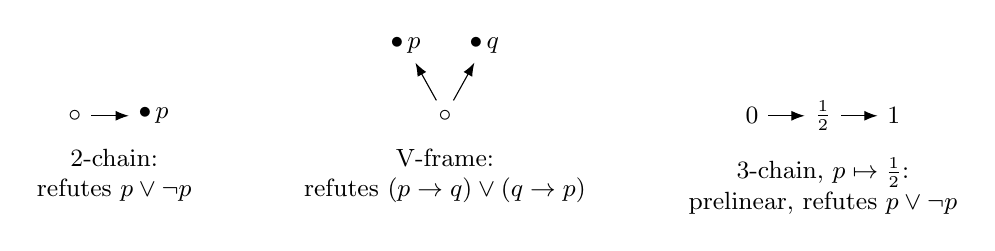
\begin{tikzpicture}[every node/.style={font=\small}, node distance=1.5mm]
\begin{scope}
  \node (r) at (0,0) {$\circ$};
  \node (l) at (1,0) {$\bullet\,p$};
  \draw[-{Latex}] (r) -- (l);
  \node[below=1mm of r, xshift=5mm, align=center]
    {2-chain:\\ refutes $p\vee\neg p$};
\end{scope}
\begin{scope}[xshift=4.2cm]
  \node (root) at (0.5,0) {$\circ$};
  \node (a) at (0,0.9) {$\bullet\,p$};
  \node (b) at (1,0.9) {$\bullet\,q$};
  \draw[-{Latex}] (root) -- (a);
  \draw[-{Latex}] (root) -- (b);
  \node[below=1mm of root, align=center]
    {V-frame:\\ refutes $(p\to q)\vee(q\to p)$};
\end{scope}
\begin{scope}[xshift=8.6cm]
  \node (z) at (0,0) {$0$};
  \node (h) at (0.9,0) {$\tfrac12$};
  \node (o) at (1.8,0) {$1$};
  \draw[-{Latex}] (z) -- (h);
  \draw[-{Latex}] (h) -- (o);
  \node[below=1mm of h, align=center]
    {3-chain, $p\mapsto\tfrac12$:\\ prelinear, refutes $p\vee\neg p$};
\end{scope}
\end{tikzpicture}
\end{center}

\begin{theorem}[Strict containments]
\leavevmode
\begin{itemize}
\item \code{intuitionistic\_strictly\_below\_lc}: prelinearity is not
  derivable in the EM-free calculus (\code{prelinearity\_not\_derivable},
  the V-frame countermodel), while it is LC-derivable as a schema member
  (\code{provableLC\_prelinearity}; axioms \code{propext} only).
\item \code{lc\_strictly\_below\_classical}: excluded middle is not
  LC-derivable --- the three-element G\"odel chain is prelinear and refutes
  it at the middle value (\code{em\_not\_derivable\_LC}) --- while it is
  classically derivable.
\end{itemize}
\end{theorem}

\begin{lstlisting}
-- Mettapedia/Logic/HOL/Semantics/KripkeHenkinCountermodel.lean
theorem em_not_derivable :
    ¬ ClosedTheorySet.Provable (Const := EMCanaryConst)
        (∅ : ClosedTheorySet EMCanaryConst) emCanaryExcludedMiddle

-- Mettapedia/Logic/HOL/Semantics/ForkedFrameCountermodel.lean
theorem prelinearity_not_derivable :
    ¬ ClosedTheorySet.Provable (Const := ForkedFrameConst)
        (∅ : ClosedTheorySet ForkedFrameConst) forkedPrelinearity

-- Mettapedia/Logic/HOL/Semantics/GoedelDummettCountermodel.lean
theorem intuitionistic_strictly_below_lc :
    (¬ ClosedTheorySet.Provable (Const := ForkedFrameConst)
        (∅ : ClosedTheorySet ForkedFrameConst) forkedPrelinearity) ∧
      ProvableLC (Base := ForkedFrameBase) (Const := ForkedFrameConst)
        (∅ : ClosedTheorySet (WithParams ForkedFrameConst)) forkedPrelinearityLC

theorem lc_strictly_below_classical :
    (¬ ProvableLC (Base := EMCanaryBase) (Const := EMCanaryConst)
        (∅ : ClosedTheorySet (WithParams EMCanaryConst)) emCanaryExcludedMiddleLC) ∧
      ClosedTheorySet.Provable (Const := WithParams EMCanaryConst)
        (EMSchema (Base := EMCanaryBase) EMCanaryConst) emCanaryExcludedMiddleLC
\end{lstlisting}

Together with the classical Henkin completeness previously mechanized in the
same development (\code{henkin\_satisfiable}), the tower is complete: three
completeness theorems, two strict containments, one calculus, one model
class.

\section{The doctrine theorem: evidence is a readout}\label{sec:doctrine}

The PLN evidence carrier \BE{} consists of pairs
$(n^+,n^-)\in[0,\infty]^2$ of positive and negative evidence.  Under the
coordinatewise order it is a \emph{frame} --- a complete Heyting algebra with
a G\"odel-style implication computed componentwise --- so evidence-valued
models of the calculus genuinely exist.  But each coordinate is a chain, and
products of chains are prelinear:

\begin{theorem}[Evidence-as-truth forces prelinearity]
$(a\himp b)\sqcup(b\himp a)=\top$ holds in \BE{}
(\code{binaryEvidence\_goedelDummett}), while excluded middle fails at the
balanced value $(1,1)$ (\code{binaryEvidence\_not\_boolean}).  Consequently
every \BE{}-valued model of the calculus --- equivalently, every pushforward
of a model along a structure-preserving map into \BE{},
\code{HeytingGeneralModel.pushforward} --- validates the LC schema
(\code{pushforward\_binaryEvidence\_validates\_lc}).
\end{theorem}

\begin{lstlisting}
-- Mettapedia/PLN/Bridges/HOL/EvidenceValuedModels.lean
theorem binaryEvidence_goedelDummett (a b : BinaryEvidence) :
    (a ⇨ b) ⊔ (b ⇨ a) = ⊤

theorem binaryEvidence_not_boolean :
    ∃ a : BinaryEvidence, a ⊔ (a ⇨ ⊥) ≠ ⊤
\end{lstlisting}

Since prelinearity is \emph{not} intuitionistically derivable
(Section~\ref{sec:strictness}), taking evidence values as primitive truth
values silently strengthens the logic to G\"odel--Dummett.  This is the
precise algebraic form of the support/evidence separation: intuitionistic
truth lives in Heyting support; graded evidence enters as a monotone
\emph{readout} of it; and if a graded, prelinear semantics is wanted on
purpose, the LC rung of the tower is its certified home.  The doctrine is
thus not a design taste but a theorem, and the tower supplies certified
semantics on both sides of it.

\section{Certified evidence readouts}\label{sec:readouts}

\paragraph{Readout interfaces.}  A readout is a monotone map
$\mu:\Omega\to Q$ from a support order into an evidence carrier
(\code{WMReadout}); an order-reflecting readout recovers support from
evidence; a \emph{separating family} $\{\mu_i\}$ jointly recovers it:
$(\forall i.\ \mu_i a\le \mu_i b)\Rightarrow a\le b$
(\code{SeparatingWMReadouts}).

\begin{theorem}[Completeness as separation]
The pointed evidence states $(M,\omega)$ --- a model with a distinguished
value, satisfaction being $\omega\le\mathrm{val}(\varphi)$ --- that model a
parameter-free theory $T$, reading formulas to crisp singleton query
strengths, form a separating family for the derivability order
$\varphi\le\psi:\Leftrightarrow\Prov_T(\varphi\to\psi)$.  In particular
$T\vdash\varphi\to\psi$ iff the strength of $\varphi$ is at most that of
$\psi$ at every such state.
\end{theorem}

\begin{lstlisting}
-- Mettapedia/PLN/Bridges/HOL/PLNHeytingHOLWorldModelBridge.lean
theorem provable_imp_iff_singletonStrengthLEOnTheory
    {T : ClosedTheorySet (WithParams Const)}
    (hT0 : ∀ ψ ∈ T, ∀ (σ : Ty Base) (k : Nat),
      NoConstOccurrence (param σ k : WithParams Const σ) ψ)
    (φ ψ : ClosedFormula (WithParams Const)) :
    ClosedTheorySet.Provable (Const := WithParams Const) T (.imp φ ψ) ↔
      singletonStrengthLEOnTheory (Base := Base) T φ ψ

noncomputable def heytingCrispSeparatingReadouts
    (T : ClosedTheorySet (WithParams Const))
    (hT0 : ∀ ψ ∈ T, ∀ (σ : Ty Base) (k : Nat),
      NoConstOccurrence (param σ k : WithParams Const σ) ψ) :
    Mettapedia.PLN.WorldModel.SeparatingWMReadouts
      {S : PointedHeytingHOL Base (WithParams Const) // stateModelsTheory T S}
      (ClosedFormula (WithParams Const)) ℝ≥0∞
      (fun φ ψ => ClosedTheorySet.Provable (Const := WithParams Const) T (.imp φ ψ))
      (· ≤ ·)
-- (instance fields mu / monotone / separating: proofs in source)
\end{lstlisting}

The completeness direction is carried by the Lindenbaum model \emph{pointed
at the antecedent itself} --- the canonical model's states are formulas, so
the separating family is definable without any further construction.  This
is the faithfulness guarantee for graded reporting: evidence comparisons
provably track derivability and cannot silently diverge from the logic.

\paragraph{Proof-relevant derivations and their evaluations.}  A
\code{DerivationTree} mirror of the calculus (with an axiom-free erasure and
\code{nonempty\_iff\_extDerivation}) supports semiring-style evaluation: the
Boolean evaluation recovers derivability
(\code{boolTreeProvable\_iff\_provable}); source ledgers
(\code{sourceIdeal}) record which hypotheses a proof used; cost spectra
(\code{costSpectrum}, \code{costUpperBounds}) grade proof effort, with
monotone transport along derivable implication up to an explicit additive
slack; and evidence grades (\code{evGrade}) land in \BE{}, aggregating over
finite bags of source-disjoint derivations by evidence addition, so ``more
independent derivations, more evidence'' is a theorem.  The same derivation
object thus admits a trust-audit reading and a graded reading --- the
provenance-semiring perspective~\cite{provenance} applied to proof theory.

\paragraph{Exactness certificates.}  For inference rules, the readout stack
supports \emph{exactness} statements: the evidence transform effected by a
rule application either equals a closed-form combination of the premise
grades or is honestly bounded by one, with exhibited lossy cases.  The first
such certificate, for modus ponens, is an equality
(\code{evGrade\_impE\_exact}); the programme of regrounding the PLN rule
families (deduction, revision, induction/abduction) as exactness or bound
certificates against this semantics is under way, with revision already
half-captured by the source-disjoint aggregation law.

\begin{lstlisting}
-- Mettapedia/PLN/Bridges/HOL/BinaryEvidenceReadout.lean
theorem evGrade_impE_exact
    (dImp : DerivationTree Const Δ (.imp φ ψ))
    (dφ : DerivationTree Const Δ φ) :
    evGrade (DerivationTree.impE dImp dφ) =
      ruleRevisionCandidate (evGrade dImp) (evGrade dφ)
\end{lstlisting}

\section{Axiom audit}\label{sec:audit}

\begin{table}[h]
\centering\footnotesize
\begin{tabular}{ll}
\toprule
Theorem & Axioms\\
\midrule
\code{HeytingSem.sound} & \code{propext}, \code{Quot.sound}\\
\code{em\_not\_derivable} & \code{propext}, \code{Quot.sound}\\
\code{ofKripkeHenkin} & \code{propext}, \code{Quot.sound}\\
\code{provableLC\_prelinearity} & \code{propext}\\
\code{provable\_iff\_heytingConsequence\_param\_free} &
  \code{propext}, \code{Classical.choice}, \code{Quot.sound}\\
\code{provableLC\_iff\_prelinearHeytingConsequence\_param\_free} &
  \code{propext}, \code{Classical.choice}, \code{Quot.sound}\\
\code{binaryEvidence\_goedelDummett} &
  \code{propext}, \code{Classical.choice}, \code{Quot.sound}\\
\code{provable\_imp\_iff\_singletonStrengthLEOnTheory} &
  \code{propext}, \code{Classical.choice}, \code{Quot.sound}\\
\bottomrule
\end{tabular}
\caption{Axiom footprints (\code{\#print axioms}).  Soundness and the
negative canaries are choice-free; completeness directions use classical
choice, as expected of Henkin-style constructions.}
\label{tab:audit}
\end{table}

\section{Related work}\label{sec:related}

Henkin's completeness for the theory of types~\cite{henkin} and Andrews's
general-models tradition~\cite{andrews} supply the classical rung and the
general-model discipline used throughout.  DeMarco and
Lipton~\cite{demarco-lipton} and Hermant and Lipton~\cite{hermant-lipton}
develop completeness and cut-elimination for intuitionistic type theory and
identify the impredicative obstruction to truth-lemma-style arguments that
our mechanization reproduces and routes around; our Lindenbaum shortcut
corresponds to their with-cut term-model observation.  G\"odel's
finite-valued systems~\cite{goedel32} and Dummett's axiomatization of
LC~\cite{dummett} ground the middle rung; the algebraic completeness
tradition for such logics goes back to Rasiowa and
Sikorski~\cite{rasiowa-sikorski}, whose enough-constants quantifier treatment
is exactly the fresh-parameter exactness used here.  Provenance semirings are
due to Green, Karvounarakis, and Tannen~\cite{provenance}.  Mechanized
completeness proofs for first-order and propositional intuitionistic systems
(e.g.~\cite{from,forster-kirst-wehr}) informed the enumeration-hypothesis
discipline of the canonical bridge; to our knowledge the mechanized
G\"odel--Dummett completeness at higher order, the strictness tower, and the
doctrine theorem are new.

\section{Conclusion and outlook}

One calculus, one model class, three certified strengths, strict
containments, and a graded readout stack whose faithfulness to derivability
is itself a theorem.  Open continuations, each scoped in the development:
completeness of the LC rung with respect to \BE{}-valued models specifically
(a quantifier-aware subdirect representation into chain products); an
enumeration-package instance unconditionalizing the canonical Kripke bridge;
the systematic regrounding of graded inference-rule families as exactness
certificates; and the agent-facing side --- using the certified readouts as
an introspection layer in which a reasoning system's confidence reports are
recomputed from proof certificates rather than stored as unaccountable
numbers, with retraction handled provenance-exactly.  The tower makes those
reports trustworthy by construction: whatever an agent says about the
strength of its beliefs, the mathematics underneath says it about
derivability too.

\begin{thebibliography}{9}\small
\bibitem{henkin} L.~Henkin. Completeness in the theory of types.
  \emph{J.\ Symbolic Logic} 15(2):81--91, 1950.
\bibitem{andrews} P.~B.~Andrews. General models, descriptions, and choice in
  type theory. \emph{J.\ Symbolic Logic} 37(2):385--394, 1972.
\bibitem{demarco-lipton} M.~DeMarco and J.~Lipton. Completeness and
  cut-elimination in the intuitionistic theory of types. \emph{J.\ Logic and
  Computation} 15(6):821--854, 2005.
\bibitem{hermant-lipton} O.~Hermant and J.~Lipton. Completeness and
  cut-elimination in the intuitionistic theory of types, part~2.
  \emph{J.\ Logic and Computation} 20(2):597--602, 2010.
\bibitem{goedel32} K.~G\"odel. Zum intuitionistischen Aussagenkalk\"ul.
  \emph{Anzeiger Akad.\ Wiss.\ Wien} 69:65--66, 1932.
\bibitem{dummett} M.~Dummett. A propositional calculus with denumerable
  matrix. \emph{J.\ Symbolic Logic} 24(2):97--106, 1959.
\bibitem{rasiowa-sikorski} H.~Rasiowa and R.~Sikorski. \emph{The Mathematics
  of Metamathematics}. PWN, 1963.
\bibitem{provenance} T.~J.~Green, G.~Karvounarakis, and V.~Tannen.
  Provenance semirings. \emph{PODS}, 31--40, 2007.
\bibitem{from} A.~H.~From. Synthetic completeness. \emph{Archive of Formal
  Proofs}, 2023.
\bibitem{forster-kirst-wehr} Y.~Forster, D.~Kirst, and D.~Wehr. Completeness
  theorems for first-order logic analysed in constructive type theory.
  \emph{J.\ Logic and Computation} 31(1):112--151, 2021.
\end{thebibliography}

\end{document}
